\documentclass{standalone}
\usepackage{tikz, ifthen}
\usepackage{amsmath}

\begin{document}

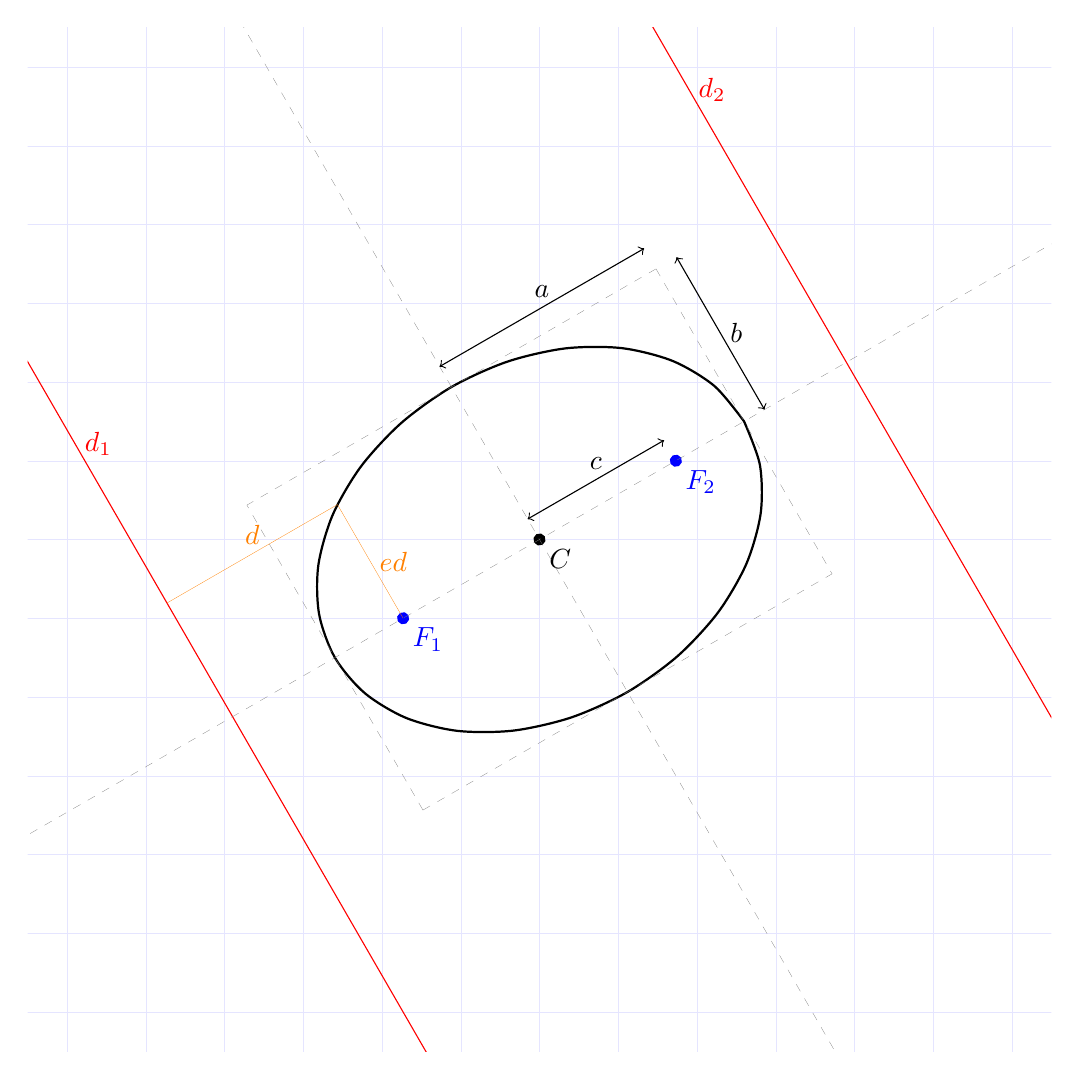
\begin{tikzpicture}
    
    % Center of the circle
    \def\xmin{-6}
    \def\xmax{6}
    \def\ymin{-6}
    \def\ymax{6}
    \def\dx{.5}
    \def\dy{.5}
    \def\xminb{\xmin-\dx}
    \def\xmaxb{\xmax+\dx}
    \def\yminb{\ymin-\dy}
    \def\ymaxb{\ymax+\dy}
    \def\xa{-2}     % x focus A 
    \def\ya{ 0}     % y focus A
    \def\xb{ 2}     % x focus B
    \def\yb{ 0}     % y focus B
    \def\xpmin{-6}
    \def\xpmax{ 6}
    \def\ypmin{-5.5}
    \def\ypmax{ 5.5}
    \def\a{3.};
    \coordinate (fa) at (\xa, \ya);
    \coordinate (fb) at (\xb, \yb);
    \def\c{sqrt((\xb-\xa)*(\xb-\xa)+(\ya-\yb)*(\ya-\yb))/2};
    \def\xc{0.5*(\xa+\xb)};
    \def\yc{0.5*(\ya+\yb)};
    \def\e{(\c/\a)}
    \def\ed{\c*(1.-\e*\e)/\e}
    \def\d{(\ed/\e)}
    \coordinate (center) at ({\xc}, {\yc});
%   \def\b{sqrt(\c*\c-\a*\a)}; % hyperbola
    \def\b{sqrt(\a*\a-\c*\c)}; % ellipses
%   \def\alpha{{atan2(\yb-\ya,\xb-\xa)}};
    \def\alpha{30}

    \clip (\xminb, \yminb) rectangle (\xmaxb, \ymaxb);

    % Draw grid
    \draw[step=1., blue!10, ultra thin] (\xmin-2, \ymin-2) grid (\xmax+2, \ymax+2); % Visible grid with lighter color

%   % Axes, x
%   \draw[->, thick, blue] (\xmin, 0) -- (\xmax, 0) node[below right] {$x$};
%   \draw[    thick, blue] (\xmin-2, 0) -- (\xmax+2, 0);
%   \draw[->, thick, blue] (0, \ymin) -- (0, \ymax) node[right] {$y$};
%   \draw[    thick, blue] (0, \ymin-2) -- (0, \ymax+2);
%   % Axis ticks
%   \foreach \x in {\xmin,..., \xmax}{
%       \ifthenelse{ \x = 0 }{}{\draw[blue] (\x, -0.1) -- (\x, +0.1) node[below=8pt, left=0pt] {\small $\x$};}
%   }
%   \foreach \y in {\ymin,..., \ymax}{
%       \ifthenelse{ \y = 0 }{}{\draw[blue] (-0.1, \y) -- (0.1, \y) node[left=4pt] {\small $\y$};}
%   }
    
    % Ellipses
    \draw[thick, black, rotate=\alpha] plot[parametric, smooth, domain=0:360] ({ \xc+\a*cos(\x)}, {\yc+\b*sin(\x)});
%   % Asymptotes
%   \draw[thick, dashed, rotate=\alpha] ({-10*\a},{-10*\b}) -- ({ 10*\a}, {10*\b});
%   \draw[thick, dashed, rotate=\alpha] ({ 10*\a},{-10*\b}) -- ({-10*\a}, {10*\b});
    % Foci
    \filldraw[blue, rotate=\alpha] ({-\c},0) circle (2pt) node[below right] {$F_1$};
    \filldraw[blue, rotate=\alpha] ({ \c},0) circle (2pt) node[below right] {$F_2$};
    \filldraw[      rotate=\alpha] (   0 ,0) circle (2pt) node[below right] {$C$};
    % Directrices
    \draw[red, rotate=\alpha] ({ \d+\xb},-10) -- ({ \d+\xb},10);
    \draw[red, rotate=\alpha] ({-\d-\xb},-10) -- ({-\d-\xb},10);
    \filldraw[red, rotate=\alpha] ({-\c-\d},4) circle (0) node[right] {$d_1$};
    \filldraw[red, rotate=\alpha] ({ \c+\d},4) circle (0) node[right] {$d_2$};
    % Semi-latus rectum
    \draw[ultra thin, orange, rotate=\alpha] ({-\c},0) -- ({-\c},{ \ed})       node[midway, right] {$ed$};
    \draw[ultra thin, orange, rotate=\alpha] ({-\c},{\ed}) -- ({-\c-\d},{\ed}) node[midway, above] {$d$};

    % Construction lines
    \draw[ultra thin, black!50, dashed, rotate=\alpha] (0,-10) -- (0,10);
    \draw[ultra thin, black!50, dashed, rotate=\alpha] (-10,0) -- (10,0);
    % Rectangle
    \draw[ultra thin, black!50, dashed, rotate=\alpha] ({-\a},{-\b}) -- ({ \a},{-\b});
    \draw[ultra thin, black!50, dashed, rotate=\alpha] ({-\a},{-\b}) -- ({-\a},{ \b});
    \draw[ultra thin, black!50, dashed, rotate=\alpha] ({ \a},{ \b}) -- ({ \a},{-\b});
    \draw[ultra thin, black!50, dashed, rotate=\alpha] ({ \a},{ \b}) -- ({-\a},{ \b});

    % Measurements
    \draw[<->, black, rotate=\alpha] (0,{   0.3})     -- ({\c},{   0.3})      node [midway, above] {$c$};
    \draw[<->, black, rotate=\alpha] (0,{\b+0.3})     -- ({\a},{\b+0.3})      node [midway, above] {$a$};
    \draw[<->, black, rotate=\alpha] ({  \a+0.3},{0}) -- ({     \a+0.3},{\b}) node [midway, right] {$b$};

%     % Axes, x'
%     \draw[->, thick, red, rotate=30] (\xmin, \yo) -- (\xmax, \yo) node[right] {$x'$};
%     \draw[->, thick, red, rotate=30] (\xo, \ymin) -- (\xo, \ymax) node[right] {$y'$};
%     \draw[    thick, red, rotate=30] (\xmin-2, 0) -- (\xmax+2, 0);
%     \draw[    thick, red, rotate=30] (0, \ymin-2) -- (0, \ymax+2);
%     % Axis thick
%     \foreach \x in {\xmin,..., \xmax}{
%         \ifthenelse{ \x = 0 }{}{\draw[red, rotate=30] (\x+\xo, \yo-0.1) -- (\x+\xo, \yo+0.1) node[below=8pt, left=0pt] {\small $\x$};}
%     }
%     \foreach \y in {\ymin,...,\ymax}{
%         \ifthenelse{ \y = 0 }{}{\draw[red, rotate=30] (\xo-0.1, \yo+\y) -- (\xo+0.1, \yo+\y) node[left=4pt] {\small $\y$};}
%     }
%     % Origin
%     \filldraw[blue] (0,0) circle (2pt) node[below=7pt, right=-13pt] {$O$};
%     \filldraw[red] (\xo,\yo) circle (2pt) node[below=7pt, right=-3pt] {$\equiv O'$};

    
\end{tikzpicture}

\end{document}
